\documentclass[10pt]{article}
\usepackage{tikz}
\usetikzlibrary{shapes.misc}
\usepackage[margin=0cm]{geometry}
\pagestyle{empty}
\tikzstyle{every node}=[cross out, draw, red]

\begin{document}

\vspace*{\fill}
\begin{center}
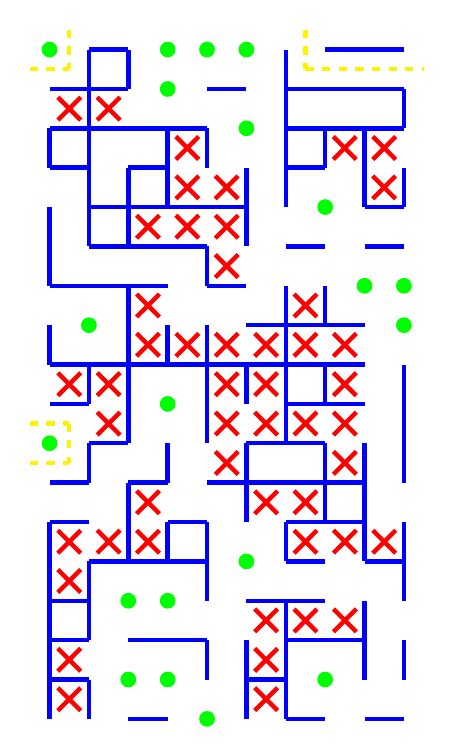
\begin{tikzpicture}[x=0.5cm, y=-0.5cm, ultra thick, blue]
% Walls
    \draw (1,0) -- (2,0);
    \draw (7,0) -- (9,0);
    \draw (0,1) -- (2,1);
    \draw (4,1) -- (5,1);
    \draw (6,1) -- (9,1);
    \draw (0,2) -- (4,2);
    \draw (6,2) -- (9,2);
    \draw (0,3) -- (1,3);
    \draw (2,3) -- (3,3);
    \draw (6,3) -- (7,3);
    \draw (1,4) -- (5,4);
    \draw (8,4) -- (9,4);
    \draw (1,5) -- (4,5);
    \draw (6,5) -- (7,5);
    \draw (8,5) -- (9,5);
    \draw (0,6) -- (3,6);
    \draw (4,6) -- (5,6);
    \draw (5,7) -- (8,7);
    \draw (0,8) -- (8,8);
    \draw (0,9) -- (1,9);
    \draw (6,9) -- (8,9);
    \draw (1,10) -- (2,10);
    \draw (5,10) -- (7,10);
    \draw (0,11) -- (1,11);
    \draw (2,11) -- (3,11);
    \draw (4,11) -- (8,11);
    \draw (0,12) -- (1,12);
    \draw (3,12) -- (4,12);
    \draw (6,12) -- (8,12);
    \draw (1,13) -- (4,13);
    \draw (6,13) -- (7,13);
    \draw (8,13) -- (9,13);
    \draw (0,14) -- (1,14);
    \draw (5,14) -- (7,14);
    \draw (0,15) -- (1,15);
    \draw (2,15) -- (4,15);
    \draw (6,15) -- (8,15);
    \draw (0,16) -- (1,16);
    \draw (5,16) -- (6,16);
    \draw (2,17) -- (3,17);
    \draw (6,17) -- (7,17);
    \draw (8,17) -- (9,17);
    \draw (0,2) -- (0,3);
    \draw (0,4) -- (0,6);
    \draw (0,7) -- (0,8);
    \draw (0,12) -- (0,17);
    \draw (1,0) -- (1,5);
    \draw (1,8) -- (1,9);
    \draw (1,10) -- (1,11);
    \draw (1,13) -- (1,15);
    \draw (1,16) -- (1,17);
    \draw (2,0) -- (2,1);
    \draw (2,3) -- (2,5);
    \draw (2,6) -- (2,10);
    \draw (2,11) -- (2,13);
    \draw (3,2) -- (3,4);
    \draw (3,7) -- (3,8);
    \draw (3,10) -- (3,11);
    \draw (3,12) -- (3,13);
    \draw (4,2) -- (4,3);
    \draw (4,5) -- (4,6);
    \draw (4,7) -- (4,10);
    \draw (4,12) -- (4,14);
    \draw (4,15) -- (4,16);
    \draw (5,3) -- (5,5);
    \draw (5,8) -- (5,9);
    \draw (5,10) -- (5,12);
    \draw (5,15) -- (5,17);
    \draw (6,0) -- (6,4);
    \draw (6,6) -- (6,10);
    \draw (6,12) -- (6,13);
    \draw (6,14) -- (6,17);
    \draw (7,2) -- (7,3);
    \draw (7,6) -- (7,7);
    \draw (7,8) -- (7,9);
    \draw (7,10) -- (7,12);
    \draw (8,2) -- (8,4);
    \draw (8,10) -- (8,13);
    \draw (8,14) -- (8,16);
    \draw (9,1) -- (9,2);
    \draw (9,3) -- (9,4);
    \draw (9,8) -- (9,11);
    \draw (9,12) -- (9,14);
    \draw (9,15) -- (9,16);
% Pillars
    \fill[green] (0,0) circle(0.2);
    \fill[green] (3,0) circle(0.2);
    \fill[green] (4,0) circle(0.2);
    \fill[green] (5,0) circle(0.2);
    \fill[green] (3,1) circle(0.2);
    \fill[green] (5,2) circle(0.2);
    \fill[green] (7,4) circle(0.2);
    \fill[green] (8,6) circle(0.2);
    \fill[green] (9,6) circle(0.2);
    \fill[green] (1,7) circle(0.2);
    \fill[green] (9,7) circle(0.2);
    \fill[green] (3,9) circle(0.2);
    \fill[green] (0,10) circle(0.2);
    \fill[green] (5,13) circle(0.2);
    \fill[green] (2,14) circle(0.2);
    \fill[green] (3,14) circle(0.2);
    \fill[green] (2,16) circle(0.2);
    \fill[green] (3,16) circle(0.2);
    \fill[green] (7,16) circle(0.2);
    \fill[green] (4,17) circle(0.2);
% Inner points in accessible cul-de-sacs
    \node at (0.5,1.5) {};
    \node at (1.5,1.5) {};
    \node at (3.5,2.5) {};
    \node at (7.5,2.5) {};
    \node at (8.5,2.5) {};
    \node at (3.5,3.5) {};
    \node at (4.5,3.5) {};
    \node at (8.5,3.5) {};
    \node at (2.5,4.5) {};
    \node at (3.5,4.5) {};
    \node at (4.5,4.5) {};
    \node at (4.5,5.5) {};
    \node at (2.5,6.5) {};
    \node at (6.5,6.5) {};
    \node at (2.5,7.5) {};
    \node at (3.5,7.5) {};
    \node at (4.5,7.5) {};
    \node at (5.5,7.5) {};
    \node at (6.5,7.5) {};
    \node at (7.5,7.5) {};
    \node at (0.5,8.5) {};
    \node at (1.5,8.5) {};
    \node at (4.5,8.5) {};
    \node at (5.5,8.5) {};
    \node at (7.5,8.5) {};
    \node at (1.5,9.5) {};
    \node at (4.5,9.5) {};
    \node at (5.5,9.5) {};
    \node at (6.5,9.5) {};
    \node at (7.5,9.5) {};
    \node at (4.5,10.5) {};
    \node at (7.5,10.5) {};
    \node at (2.5,11.5) {};
    \node at (5.5,11.5) {};
    \node at (6.5,11.5) {};
    \node at (0.5,12.5) {};
    \node at (1.5,12.5) {};
    \node at (2.5,12.5) {};
    \node at (6.5,12.5) {};
    \node at (7.5,12.5) {};
    \node at (8.5,12.5) {};
    \node at (0.5,13.5) {};
    \node at (5.5,14.5) {};
    \node at (6.5,14.5) {};
    \node at (7.5,14.5) {};
    \node at (0.5,15.5) {};
    \node at (5.5,15.5) {};
    \node at (0.5,16.5) {};
    \node at (5.5,16.5) {};
% Entry-exit paths without intersections
    \draw[dashed, yellow] (-0.5,0.5) -- (0.5,0.5);
    \draw[dashed, yellow] (6.5,0.5) -- (9.5,0.5);
    \draw[dashed, yellow] (-0.5,9.5) -- (0.5,9.5);
    \draw[dashed, yellow] (-0.5,10.5) -- (0.5,10.5);
    \draw[dashed, yellow] (0.5,-0.5) -- (0.5,0.5);
    \draw[dashed, yellow] (0.5,9.5) -- (0.5,10.5);
    \draw[dashed, yellow] (6.5,-0.5) -- (6.5,0.5);
\end{tikzpicture}
\end{center}
\vspace*{\fill}

\end{document}
